%---------------------------------------------------------
%	PRESENTATION BODY SLIDES
%---------------------------------------------------------
\section{INFORMATION TEORY} % Note all sections and subsections are automatically placed in your table of contents

%------------------------------------------------
\begin{frame}
    \frametitle{Catatan 1}
       \vspace*{-0.5cm}
  \begin{columns}[T]
  \small
    \begin{column}{0.5\textwidth}
        \begin{itemize}
            \item Entropi \cite{djordjevic2019physical}\\
                \begin{itemize}
                \tiny \justifying                
                    \item[$\Rightarrow$] Entropi adalah ukuran dari ketidakpastian atau kekacauan dalam suatu sistem atau distribusi probabilitas.
                    \item[$\Rightarrow$]  Dalam teori informasi, entropi digunakan untuk mengukur seberapa banyak informasi yang terkandung dalam suatu variabel acak. 
                    \item[$\Rightarrow$] Entropi memiliki keterkaitan dengan konsep ketidakpastian dalam sistem, di mana semakin tinggi entropi suatu sistem, semakin tinggi pula ketidakpastian atau kekacauan dalam sistem tersebut.
                \end{itemize}
            \item Conditional Entropy\\
                \begin{itemize}
                \tiny \justifying
                    \item[$\Rightarrow$] \textit{Conditional entropy} adalah ukuran ketidakpastian yang tersisa pada input saluran setelah output saluran diterima.
                    \item[$\Rightarrow$]  \textit{Conditional entropy} mengukur seberapa banyak informasi yang masih tidak diketahui pada input saluran setelah melihat output saluran.
                    \item[$\Rightarrow$] \textit{Conditional entropy} dapat diukur melalui persamaan
                        \begin{equation}
                            H(Y|X) = -\sum_{x \in X} p(x) \sum_{y \in Y}  \, p(y|x) \log p(y|x),
                        \end{equation}
                     di mana $p(x,y)$ adalah \textit{joint distribution} dari input dan output saluran.
                \end{itemize}
        \end{itemize}
    \end{column}

   \begin{column}{0.5\textwidth}
        \begin{itemize}
            \item Relative Entropy \cite{wolfowitz2012coding}\\
                \begin{itemize}
                \tiny \justifying                
                    \item[$\Rightarrow$] Relative Entropy, juga dikenal sebagai Kullback-Leibler (KL) distance, adalah ukuran jarak antara dua distribusi probabilitas.
                    \item[$\Rightarrow$]   Relative Entropy mengukur ketidakefisiesi antara dua jarak distribusi probabilitas dengan mengasumsikan distribusi q(x) ketika distribusi sebenarnya adalah p(x). 
                    \item[$\Rightarrow$] Relative Entropy dapat diukur melalui persamaan 
                        \begin{equation}
                            D(p||q) = \sum p(x) \log\left(\frac{p(x)}{q(x)}\right).
                        \end{equation}
                \end{itemize}
            \item Mutual Information \cite{djordjevic2019physical}\\
                \begin{itemize}
                \tiny \justifying
                    \item[$\Rightarrow$] Mutual Information adalah ukuran seberapa banyak informasi yang dikandung oleh satu variabel acak terkait dengan variabel acak lainnya..
                    \item[$\Rightarrow$]  Mutual Information mengukur seberapa banyak informasi yang diketahui pada input saluran setelah melihat output saluran.
                    \item[$\Rightarrow$]Mutual Information dapat diukur melalui persamaan
                        \begin{equation}
                           I(X;Y) = H(X) - H(X|Y),
                        \end{equation}
                     di mana $H(X)$ adalah entropy dari output saluran dan $H(X|Y)$ adalah conditional entropy.
                \end{itemize}
        \end{itemize}
    \end{column}
  \end{columns}   
\end{frame}

\begin{frame}
    \frametitle{Catatan 2}
       \vspace*{-0.5cm}
  \begin{columns}[T]
  \small
    \begin{column}{0.5\textwidth}
        \begin{itemize}
            \item Channel Capacity\cite{djordjevic2019physical}\\
                \begin{itemize}
                \tiny \justifying                
                    \item[$\Rightarrow$] Channel Capacity adalah batasan penting pada tingkat data yang dapat dicapai oleh skema modulasi dan pengkodean apa pun. 
                    \item[$\Rightarrow$]  Ini juga dapat digunakan untuk membandingkan skema modulasi dan pengkodean yang berbeda dalam hal jarak mereka dari kurva kapasitas saluran maksimum. 
                    \item[$\Rightarrow$] Persamaan channel capacity yaitu 
                        \begin{equation}
                            C = \log_2 M + (1 - P_s) \log_2(1 - P_s) + P_s \log_2\left(\frac{P_s}{M - 1}\right).
                        \end{equation}
                    \item[$\Rightarrow$] Kapasitas saluran, \( C \), mengukur jumlah maksimum informasi yang dapat dikirimkan melalui suatu saluran (misalnya, kabel) yang didefinisikan sebagai berikut
                    \begin{equation}
                        C = \max_{P(X)} I(X, Y),
                    \end{equation}
                    di mana \( X \) adalah masukan ke saluran dan \( Y \) adalah keluaran.

                \end{itemize}
        \end{itemize}
    \end{column}

    \begin{column}{0.5\textwidth}
         \begin{itemize}
            \item Information Capacity Theorem\\
                \begin{itemize}
                \tiny \justifying
                    \item[$\Rightarrow$] Teorema Kapasitas Informasi menyatakan kondisi di mana suatu sumber diskrit tanpa memori dengan entropi $H(S)$ dan kapasitas $C$ dapat mentransmisikan informasi melalui saluran dengan probabilitas kesalahan yang sangat kecil.
                    \item[$\Rightarrow$] Informasi  pada sistem klasik ataupun kuantum  diukur dari jumlah minimal komunikasi pada saat penyampaiannya \cite{cerf1996quantum}.
                    \item[$\Rightarrow$] Menurut Slepian \& Wolf: jumlah informasi yang diperlukan untuk memperoleh pengetahuan penuh diberikan oleh sejumlah yang disebut \textbf{Conditional Entropy}.
                    \item[$\Rightarrow$] Menurut Shannon: jumlah informasi dari suatu sumber adalah memori yang diperlukan untuk merepresentasikan keluarannya dan diberikan oleh \textbf{entropi} sumber tersebut \cite{cerf1996quantum}.
                    \item[$\Rightarrow$] Kriteria utama teorema adalah bahwa rasio entropi sumber terhadap waktu simbol ($\frac{H(S)}{T}$) harus kurang dari atau sama dengan rasio kapasitas saluran terhadap waktu saluran ($\frac{C}{T_c}$).
                    \item[$\Rightarrow$] Jika $\frac{H(S)}{T} \leq \frac{C}{T_c}$, maka skema pengkodean dapat dibangun untuk mentransmisikan keluaran sumber melalui saluran dengan tingkat kesalahan yang sangat kecil.
                    \item[$\Rightarrow$] Kondisi rasio yang ditetapkan oleh teorema mengindikasikan bahwa penggunaan waktu dan kapasitas saluran harus seimbang. Jika kriteria terpenuhi, skema pengkodean efisien dapat dikembangkan untuk mentransmisikan informasi melalui saluran dengan probabilitas kesalahan yang sangat rendah.
                \end{itemize}
            \end{itemize}    
    \end{column}
   \end{columns}   
\end{frame}

\begin{frame}
    \frametitle{Catatan 3}
       \vspace*{-0.5cm}
  \begin{columns}[T]
  \small
    \begin{column}{0.5\textwidth}
        \begin{itemize} \justifying \tiny
            \item Joint Entropy\\
                Joint Entropy merupakan total ketidakpastian tentang pasangan (X, Y), yang dapat dituliskan sebagai: 
                    \begin{equation}
                        H(X, Y) \equiv -\sum_{x, y} p(x, y) \log p(x, y).
                    \end{equation}
            \item Conditional Entropy\\
                Entropy Kondisional (Conditional Entropy) merupakan ketidakpastian pada rata-rata X diberikan Y dan nilainya selalu non-negatif dapat dituliskan sebagai:
                    \begin{equation}
                         H(X|Y) \equiv H(X, Y) - H(Y).
                    \end{equation}
            \item Mutual Entropy\\
                Mutual Entropy merupakan informasi yang terkandung pada X dan Y yang dapat dituliskan sebagai:
                    \begin{equation}
                         H(X:Y) \equiv H(X) + H(Y) - H(X, Y).
                    \end{equation}
                
        \end{itemize}
    \end{column}

    \begin{column}{0.5\textwidth}
         \begin{itemize} \tiny \justifying
            \item -\\
                \begin{itemize}
                \tiny \justifying
                    \item[$\Rightarrow$] 
                \end{itemize}
            \end{itemize}    
    \end{column}
   \end{columns}   
\end{frame}

% \begin{frame}
%     \frametitle{Slepian–Wolf Bound}
%        \vspace{-0.5cm}
%   \begin{columns}
%   \small
%     \begin{column}{0.5\textwidth}
%         \begin{itemize} 
%              \begin{figure}
%              \centering
%              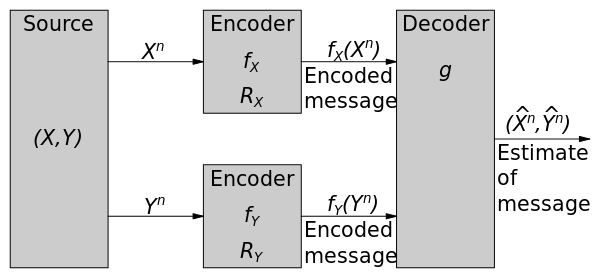
\includegraphics[width=0.8\textwidth]{gambar/BASIC/SlepianWolfEncoderDecoder.png}
%              \captionsetup{font=tiny, justification=justified,width=1\textwidth}
%              \captionof{figure}{Dua sumber distribusi random X dan Y yang melalui encoder decoder.}
%              \label{fig:encoderdecoderslepianwolf}
%             \end{figure}
%     \justifying \tiny \vspace{-0.5cm}
%             \item Slepian–Wolf bound adalah batasan entropi yang menentukan jumlah bit minimum yang dibutuhkan untuk mengkodekan dua sumber data yang berkorelasi secara lossless yang ditemukan oleh David Slepian dan Jack Wolf pada tahun 1973.
%             \item Batasan ini menyatakan bahwa untuk mengkodekan dua sumber data yang berkorelasi secara lossless, laju bit total harus setidaknya sama dengan jumlah entropi sumber individu dikurangi informasi bersama.
%             \item Jika dua sumber data berkorelasi secara kuat, maka informasi yang diperlukan untuk mengkodekan satu sumber data dapat dikurangi dengan menggunakan informasi dari sumber data lainnya. 
    
%         \end{itemize}
%     \end{column}

%     \begin{column}{0.5\textwidth}

%        \tiny \justifying
%              \begin{figure}
%              \centering
%              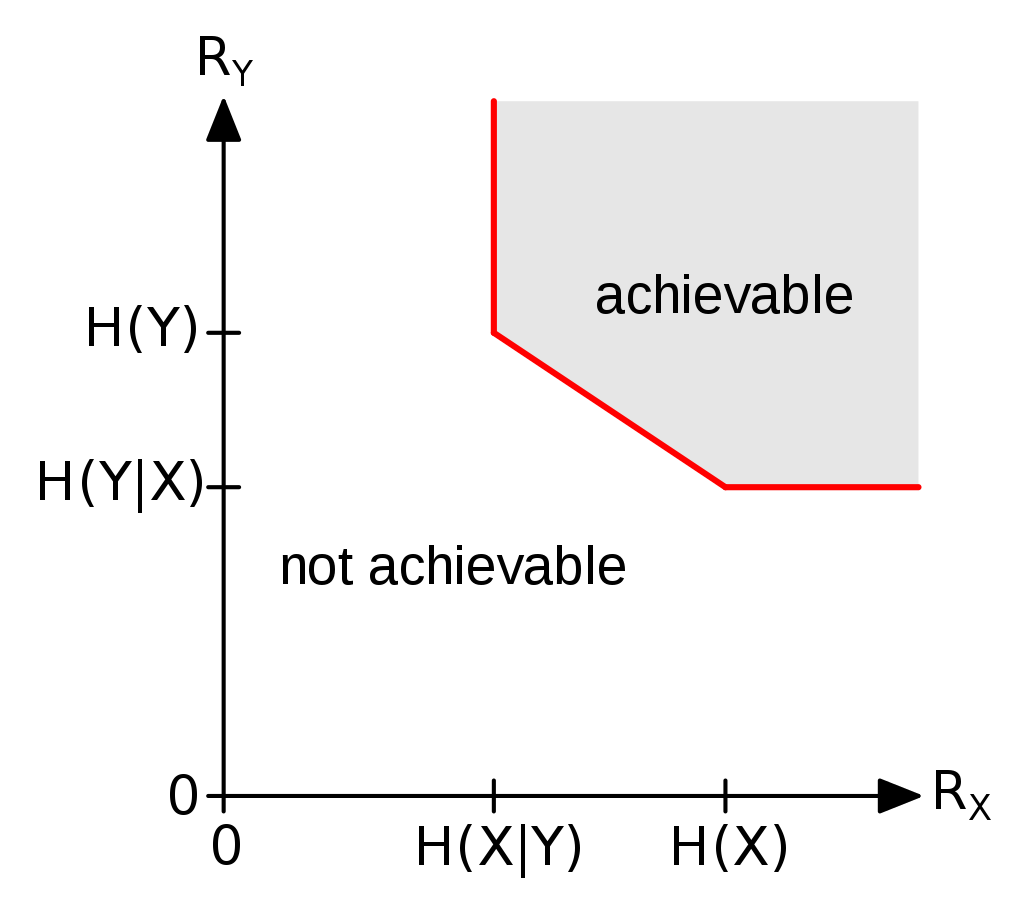
\includegraphics[width=0.5\textwidth]{gambar/BASIC/SlepianWolfPlot.png}
%              \captionsetup{font=tiny, justification=justified,width=1\textwidth}
%              \captionof{figure}{Batas tingkat lossless coding pada dua sumber X dan Y.}
%              \label{fig:encoderdecoderslepianwolf}
%             \end{figure} \vspace{-0.8cm}
%                 \begin{align*}
%                     R_X &\geq H(X|Y) \\
%                     R_Y &\geq H(Y|X) \\
%                     R_X + R_Y &\geq H(X,Y)
%                 \end{align*}
%         Sumber catatan \firstcite{slepian1973noiseless}
  
%     \end{column}
%    \end{columns}   
% \end{frame}

 
%---------------------------------------------------------
%	PRESENTATION BODY SLIDES
%---------------------------------------------------------


%------------------------------------------------
\begin{frame}
    \frametitle{INTRODUCTION 1}
       \vspace*{-0.5cm}
  \begin{columns}[T]
  \small
    \begin{column}{0.5\textwidth}
        \begin{itemize}\tiny \justifying
            \item \textbf{Deskripsi Umum Quantum Information Theory:}
            \begin{itemize}\tiny \justifying
            \item Memberikan deskripsi konsisten tentang entanglement kuantum.
            \item Paralel dengan teori informasi klasik (Shannon) namun berbasis sepenuhnya pada matriks densitas.
            \end{itemize}
            
            \item \textbf{Perbedaan dengan Teori Shannon:}
            \begin{itemize}\tiny \justifying
            \item Berfokus pada matriks densitas, bukan distribusi probabilitas seperti dalam teori Shannon.
            \item Menemukan bahwa entropi kondisional bisa negatif dalam sistem terkait kuantum, seperti pasangan Einstein-Podolsky-Rosen (EPR).
            \end{itemize}
            
            \item \textbf{Penggunaan Density Matrices:}
            \begin{itemize}\tiny \justifying
            \item Negatifnya entropi kuantum dapat ditelusuri kembali ke matriks densitas kondisional yang memiliki nilai eigen lebih besar dari satu.
            \item Menggunakan "mutual" density matrix untuk mendefinisikan mutual quantum entropy atau "mutual entanglement."
            \end{itemize}

        \end{itemize}
    \end{column}

   \begin{column}{0.5\textwidth}
        \begin{itemize}\tiny \justifying
            \item \textbf{Hubungan antara Korelasi Klasik dan Entanglement Kuantum:}
            \begin{itemize}\tiny \justifying
            \item Penjelasan terpadu tentang korelasi klasik dan entanglement kuantum.
            \item Entanglement kuantum dapat dianggap sebagai "super-korelasi" yang dapat menghasilkan korelasi klasik saat mempertimbangkan sistem ternary atau lebih besar.
            \end{itemize}
            
            \item \textbf{Implikasi Quantum Information Theory:}
            \begin{itemize}\tiny \justifying
            \item Quantum information theory memiliki implikasi potensial terhadap fondasi konseptual mekanika kuantum.
            \item Dasar pemahaman yang tepat untuk bidang-bidang baru seperti komputasi kuantum, komunikasi kuantum, dan kriptografi kuantum.
            \end{itemize}
            
            \item \textbf{Tantangan dalam Quantum Information Processing:}
            \begin{itemize}\tiny \justifying
            \item Quantum information processing melibatkan qubits, tidak seperti bits dalam klasik, dengan hukum kuantum yang berbeda.
            \item Qubits dapat ada dalam superposisi kuantum, konsep yang sepenuhnya berbeda dari mekanika klasik.
            \end{itemize}
        \end{itemize}
    \end{column}
  \end{columns}   
\end{frame}

\begin{frame}
    \frametitle{INTRODUCTION 2}
       \vspace*{-0.5cm}
  \begin{columns}[T]
  \small
    \begin{column}{0.5\textwidth}
        \begin{itemize}\tiny \justifying
            \item \textbf{Sifat Density Matrices dan Entropi von Neumann:}
            \begin{itemize}\tiny \justifying
            \item Matriks densitas Persamaan \ref{Matriks densitas} sebagai konstruksi matematika sentral dalam teori informasi kuantum.
            \item Entropi von Neumann Persamaan \ref{Entropi von Neumann} diperkenalkan dalam mekanika kuantum, terkait dengan entropi Boltzmann-Gibbs-Shannon Persamaan \ref{entropi Boltzmann-Gibbs-Shannon} pada situasi klasik tertentu.
                \begin{equation}
                    S(p) = -\text{Tr}(p \log p)
                    \label{Entropi von Neumann}
                \end{equation}

                \begin{equation}
                    H(p) = -\sum_i P_i \log P_i
                    \label{entropi Boltzmann-Gibbs-Shannon}
                \end{equation}
                
                \begin{equation}
                   \rho{A|B}=\rho_{AB}(1_A\bigotimes\rho_B)^{-1}
                    \label{}
                \end{equation}
            \end{itemize}
            
            \item \textbf{Perbandingan dengan Teori Informasi Klasik:}
            \begin{itemize}\tiny \justifying
            \item Konsep probabilitas kondisional di teori informasi klasik dan definisi entropi kondisional.
            \item Perbandingan dengan teori informasi kuantum yang menghilangkan fasa kuantum dengan menggabungkan probabilitas kuantum ke dalam rumus klasik.
            \end{itemize}

        \end{itemize}
    \end{column}

   \begin{column}{0.5\textwidth}
        \begin{itemize}\tiny \justifying
            \item \textbf{Hubungan antara Korelasi Klasik dan Entanglement Kuantum:}

            
        \end{itemize}
    \end{column}
  \end{columns}   
\end{frame}
% \begin{frame}
%     \frametitle{QUANTUM INFORMATION THEORY}
%        \vspace*{-0.5cm}
%   \begin{columns}[T]
%   \small
%     \begin{column}{0.5\textwidth}
%         \begin{itemize}
%             \item Entropi \cite{djordjevic2019physical}\\
%                 \begin{itemize}
%                 \tiny \justifying                
%                     \item[$\Rightarrow$] Entropi adalah ukuran dari ketidakpastian atau kekacauan dalam suatu sistem atau distribusi probabilitas.
%                     \item[$\Rightarrow$]  Dalam teori informasi, entropi digunakan untuk mengukur seberapa banyak informasi yang terkandung dalam suatu variabel acak. 
%                     \item[$\Rightarrow$] Entropi memiliki keterkaitan dengan konsep ketidakpastian dalam sistem, di mana semakin tinggi entropi suatu sistem, semakin tinggi pula ketidakpastian atau kekacauan dalam sistem tersebut.
%                 \end{itemize}
%             \item Conditional Entropy\\
%                 \begin{itemize}
%                 \tiny \justifying
%                     \item[$\Rightarrow$] \textit{Conditional entropy} adalah ukuran ketidakpastian yang tersisa pada input saluran setelah output saluran diterima.
%                     \item[$\Rightarrow$]  \textit{Conditional entropy} mengukur seberapa banyak informasi yang masih tidak diketahui pada input saluran setelah melihat output saluran.
%                     \item[$\Rightarrow$] \textit{Conditional entropy} dapat diukur melalui persamaan
%                         \begin{equation}
%                             H(Y|X) = -\sum_{x \in X} p(x) \sum_{y \in Y}  \, p(y|x) \log p(y|x),
%                         \end{equation}
%                      di mana $p(x,y)$ adalah \textit{joint distribution} dari input dan output saluran.
%                 \end{itemize}
%         \end{itemize}
%     \end{column}

%    \begin{column}{0.5\textwidth}
%         \begin{itemize}
%             \item Relative Entropy \cite{wolfowitz2012coding}\\
%                 \begin{itemize}
%                 \tiny \justifying                
%                     \item[$\Rightarrow$] Relative Entropy, juga dikenal sebagai Kullback-Leibler (KL) distance, adalah ukuran jarak antara dua distribusi probabilitas.
%                     \item[$\Rightarrow$]   Relative Entropy mengukur ketidakefisiesi antara dua jarak distribusi probabilitas dengan mengasumsikan distribusi q(x) ketika distribusi sebenarnya adalah p(x). 
%                     \item[$\Rightarrow$] Relative Entropy dapat diukur melalui persamaan 
%                         \begin{equation}
%                             D(p||q) = \sum p(x) \log\left(\frac{p(x)}{q(x)}\right).
%                         \end{equation}
%                 \end{itemize}
%             \item Mutual Information \cite{djordjevic2019physical}\\
%                 \begin{itemize}
%                 \tiny \justifying
%                     \item[$\Rightarrow$] Mutual Information adalah ukuran seberapa banyak informasi yang dikandung oleh satu variabel acak terkait dengan variabel acak lainnya..
%                     \item[$\Rightarrow$]  Mutual Information mengukur seberapa banyak informasi yang diketahui pada input saluran setelah melihat output saluran.
%                     \item[$\Rightarrow$]Mutual Information dapat diukur melalui persamaan
%                         \begin{equation}
%                            I(X;Y) = H(X) - H(X|Y),
%                         \end{equation}
%                      di mana $H(X)$ adalah entropy dari output saluran dan $H(X|Y)$ adalah conditional entropy.
%                 \end{itemize}
%         \end{itemize}
%     \end{column}
%   \end{columns}   
% \end{frame}

\begin{frame}
    \frametitle{CORRELATION VERSUS ENTANGLEMENT 1}
       \vspace*{-0.5cm}
  \begin{columns}[T]
  \small
    \begin{column}{0.5\textwidth}
        \begin{figure}
             \centering
             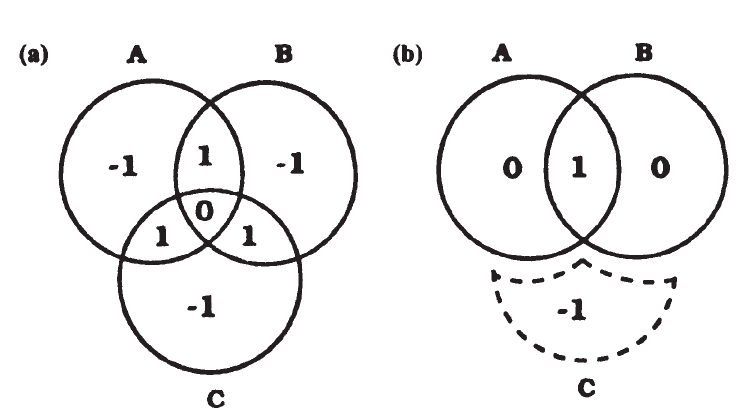
\includegraphics[width=1\textwidth]{gambar/DIAGRAM/EPR-Triplet.png}
             \captionsetup{font=tiny, justification=justified,width=1\textwidth}
             \captionof{figure}{(a) Diagram entropi ternary untuk sebuah "EPR triplet". (b) Diagram entropi untuk subsistem AB tanpa kondisi pada C.}
             \label{fig:EPR-Triplet}
        \end{figure}
        \begin{itemize} \tiny \justifying
        \vspace{-0.6 cm}
            \item[$\Rightarrow$] Fungsi Negative Conditional Entropy\\
                Dalam konteks sistem kuantum komposit yang tidak diketahui, konsep entropi kondisional negatif terbukti sangat berguna dalam menjelaskan sistem kuantum yang terdiri dari beberapa bagian, serta memberikan pemahaman baru tentang pembentukan korelasi klasikal dari \textit{quantum entanglement}.
        \end{itemize}
    \end{column}

   \begin{column}{0.5\textwidth}
        \begin{itemize} \tiny \justifying
            \item[$\Rightarrow$] Sistem EPR-triplet\\
                Dalam contoh tertentu, perlu mempertimbangkan sistem tiga partikel ABC dalam keadaan GHZ (atau "EPR-triplet"). Keadaan ini dapat dijelaskan sebagai 
                    \begin{equation}
                        \ket{\psi_{ABC}}=\frac{1}{\sqrt{2}}(\ket{000}+\ket{111}).
                    \end{equation}
            \item[$\Rightarrow$] Entangled state\\
                Dalam keadaan murni (entangled), entropi gabungan adalah \(S(ABC) = 0\). Diagram entropi ternary yang sesuai dari ABC Gambar \ref{fig:EPR-Triplet} menunjukkan bahwa \textit{ternary mutual entropy} 
                    \begin{equation}
                        S(A:B:C) = S(A)+S(B)+S(C)-S(AB)-S(AC)-S(BC)+S(ABC)
                    \end{equation}
                menghilang, yang merupakan hal umum untuk sistem tiga partikel yang sepenuhnya ter-\textit{entangled}.
            \item[$\Rightarrow$] Density matrix  subsistem AB\\
                Ketika kita melacak derajat kebebasan yang terkait dengan C, maka matriks densitas marginal untuk subsistem AB menjadi
                    \begin{equation}
                        \rho_{AB}=\text{Tr}_c[\rho_{ABc}]=\frac{1}{2}(\ket{00}\bra{00}+\ket{11}\bra{11}),
                    \end{equation} 
                yang sesuai dengan sistem klasik yang berkorelasi.
        \end{itemize}
    \end{column}
  \end{columns}   
\end{frame}

\begin{frame}
    \frametitle{CORRELATION VERSUS ENTANGLEMENT 2}
       \vspace*{-0.5cm}
  \begin{columns}[T]
  \small
    \begin{column}{0.5\textwidth}
        \begin{itemize}  \tiny \justifying
            \item[$\Rightarrow$] Teori Shannon\\
                Ini berarti bahwa jika kita mengabaikan keberadaan C, A dan B berkorelasi dalam arti teori Shannon.
            \item[$\Rightarrow$] Tracing over\\
                Operasi "tracing over" yang diilustrasikan menunjukkan penciptaan korelasi klasikal dari quantum entanglement. Ini penting dalam deskripsi proses pengukuran yang diusulkan, di mana A dan B mewakili dua bagian dari alat pengukur, sedangkan C adalah sistem kuantum yang diukur.
            \item[$\Rightarrow$] Korelasi A dan B\\
                Subsistem AB tanpa kondisi pada C menjadi tidak dapat dibedakan dari himpunan statistik yang disiapkan dengan jumlah yang sama dari keadaan \(|100\rangle\) dan \(|111\rangle\). Oleh karena itu, A dan B berkorelasi dalam arti teori Shannon jika C diabaikan.
            \item[$\Rightarrow$] Measurement\\
                Fitur ini sentral dalam deskripsi proses pengukuran yang diusulkan, di mana A dan B mewakili dua bagian dari alat pengukur, sedangkan C adalah sistem kuantum yang diukur. Entropi dari C bersyarat pada AB, \(S(C|AB)\), adalah negatif dan sama dengan -1 bit, sehingga menyeimbangkan \(S(AB)\) untuk menghasilkan entropi gabungan yang menghilang.
        \end{itemize}
    \end{column}

   \begin{column}{0.5\textwidth}
        \begin{itemize} \tiny \justifying
            \item[$\Rightarrow$] Joint Entropy\\  
                Sebagaimana diharapkan dalam konteks kuantum entanglement antara AB dan C yang di notasikan sebagai
                \begin{equation}
                    S(ABC) =S(AB) +S(C|AB) =0.
                    \label{persamaan S(ABC)}
                \end{equation}
            \item \small Simpulan\\
                \begin{itemize}\tiny \justifying
                    \item[$\Rightarrow$] Dalam Persamaan \ref{persamaan S(ABC)} bahwa interpretasi informasi-teoretik dari entanglement membuka jalan menuju model pengukuran yang alami, unitary, dan kausal, tanpa asumsi tentang runtuhnya fungsi gelombang, sambil menyiratkan semua hasil yang sudah dikenal dari mekanika kuantum probabilitas konvensional.
                    \item[$\Rightarrow$] Kerangka kerja yang sama juga dapat digunakan untuk menginterpretasikan pengamatan korelasi klasikal antara alat pengukur yang terjadi dalam pengukuran pasangan EPR, dan memberikan pencerahan baru pada paradoks kuantum.
                \end{itemize}
            \item \small Sumber\\
                \tiny Sumber catatan \firstcite{cerf1997negative}
        \end{itemize}
    \end{column}
  \end{columns}   
\end{frame}


